%% LyX 2.3.3 created this file.  For more info, see http://www.lyx.org/.
%% Do not edit unless you really know what you are doing.
\documentclass[english]{beamer}
\usepackage[T1]{fontenc}
\usepackage[latin9]{inputenc}
\setcounter{secnumdepth}{3}
\setcounter{tocdepth}{3}
\usepackage{babel}
\usepackage{amsmath}
\usepackage{stmaryrd}
\usepackage{graphicx}
\usepackage[all]{xy}
\ifx\hypersetup\undefined
  \AtBeginDocument{%
    \hypersetup{unicode=true,pdfusetitle,
 bookmarks=true,bookmarksnumbered=false,bookmarksopen=false,
 breaklinks=false,pdfborder={0 0 1},backref=false,colorlinks=true}
  }
\else
  \hypersetup{unicode=true,pdfusetitle,
 bookmarks=true,bookmarksnumbered=false,bookmarksopen=false,
 breaklinks=false,pdfborder={0 0 1},backref=false,colorlinks=true}
\fi

\makeatletter
%%%%%%%%%%%%%%%%%%%%%%%%%%%%%% Textclass specific LaTeX commands.
% this default might be overridden by plain title style
\newcommand\makebeamertitle{\frame{\maketitle}}%
% (ERT) argument for the TOC
\AtBeginDocument{%
  \let\origtableofcontents=\tableofcontents
  \def\tableofcontents{\@ifnextchar[{\origtableofcontents}{\gobbletableofcontents}}
  \def\gobbletableofcontents#1{\origtableofcontents}
}
\newenvironment{lyxcode}
  {\par\begin{list}{}{
    \setlength{\rightmargin}{\leftmargin}
    \setlength{\listparindent}{0pt}% needed for AMS classes
    \raggedright
    \setlength{\itemsep}{0pt}
    \setlength{\parsep}{0pt}
    \normalfont\ttfamily}%
   \def\{{\char`\{}
   \def\}{\char`\}}
   \def\textasciitilde{\char`\~}
   \item[]}
  {\end{list}}

%%%%%%%%%%%%%%%%%%%%%%%%%%%%%% User specified LaTeX commands.
\usetheme[secheader]{Boadilla}
\usecolortheme{seahorse}
\title[Equivalence of functions under laws]{Equivalence of typeclass methods under laws}
\subtitle{Why flatMap is "equivalent" to flatten and map}
\author{Sergei Winitzki}
\date{2021-05-08}
\institute[ABTB]{Academy by the Bay}
\setbeamertemplate{headline}{} % disable headline at top
\setbeamertemplate{navigation symbols}{} % disable navigation bar at bottom
\usepackage[all]{xy} % xypic
%\makeatletter
% Macros to assist LyX with XYpic when using scaling.
\newcommand{\xyScaleX}[1]{%
\makeatletter
\xydef@\xymatrixcolsep@{#1}
\makeatother
} % end of \xyScaleX
\makeatletter
\newcommand{\xyScaleY}[1]{%
\makeatletter
\xydef@\xymatrixrowsep@{#1}
\makeatother
} % end of \xyScaleY

% Double-stroked fonts to replace the non-working \mathbb{1}.
\usepackage{bbold}
\DeclareMathAlphabet{\bbnumcustom}{U}{BOONDOX-ds}{m}{n} % Use BOONDOX-ds or bbold.
\newcommand{\custombb}[1]{\bbnumcustom{#1}}
% The LyX document will define a macro \bbnum{#1} that calls \custombb{#1}.

\usepackage{relsize} % make math symbols larger or smaller
\usepackage{stmaryrd} % some extra symbols such as \fatsemi
% Note: using \forwardcompose inside a \text{} will cause a LaTeX error!
\newcommand{\forwardcompose}{\hspace{1.5pt}\ensuremath\mathsmaller{\fatsemi}\hspace{1.5pt}}


% Make underline green.
\definecolor{greenunder}{rgb}{0.1,0.6,0.2}
%\newcommand{\munderline}[1]{{\color{greenunder}\underline{{\color{black}#1}}\color{black}}}
\def\mathunderline#1#2{\color{#1}\underline{{\color{black}#2}}\color{black}}
% The LyX document will define a macro \gunderline{#1} that will use \mathunderline with the color `greenunder`.
%\def\gunderline#1{\mathunderline{greenunder}{#1}} % This is now defined by LyX itself with GUI support.

% Scala syntax highlighting. See https://tex.stackexchange.com/questions/202479/unable-to-define-scala-language-with-listings
%\usepackage[T1]{fontenc}
%\usepackage[utf8]{inputenc}
%\usepackage{beramono}
%\usepackage{listings}
% The listing settings are now supported by LyX in a separate section "Listings".
\usepackage{xcolor}

\definecolor{scalakeyword}{rgb}{0.16,0.07,0.5}
\definecolor{dkgreen}{rgb}{0,0.6,0}
\definecolor{gray}{rgb}{0.5,0.5,0.5}
\definecolor{mauve}{rgb}{0.58,0,0.82}
\definecolor{aqua}{rgb}{0.9,0.96,0.999}
\definecolor{scalatype}{rgb}{0.2,0.3,0.2}

\makeatother

\usepackage{listings}
\lstset{language=Scala,
morekeywords={{scala}},
otherkeywords={=,=>,<-,<\%,<:,>:,\#,@,:,[,],.,???},
keywordstyle={\color{scalakeyword}},
morekeywords={[2]{String,Short,Int,Long,Char,Boolean,Double,Float,BigDecimal,Seq,Map,Set,List,Option,Either,Future,Vector,Range,IndexedSeq,Try,true,false,None,Some,Left,Right,Nothing,Any,Array,Unit,Iterator,Stream}},
keywordstyle={[2]{\color{scalatype}}},
frame=tb,
aboveskip={1.5mm},
belowskip={0.5mm},
showstringspaces=false,
columns=fullflexible,
keepspaces=true,
basicstyle={\smaller\ttfamily},
extendedchars=true,
numbers=none,
numberstyle={\tiny\color{gray}},
commentstyle={\color{dkgreen}},
stringstyle={\color{mauve}},
frame=single,
framerule={0.0mm},
breaklines=true,
breakatwhitespace=true,
tabsize=3,
framexleftmargin={0.5mm},
framexrightmargin={0.5mm},
xleftmargin={1.5mm},
xrightmargin={1.5mm},
framextopmargin={0.5mm},
framexbottommargin={0.5mm},
fillcolor={\color{aqua}},
rulecolor={\color{aqua}},
rulesepcolor={\color{aqua}},
backgroundcolor={\color{aqua}},
mathescape=false,
extendedchars=true}
\renewcommand{\lstlistingname}{Listing}

\begin{document}
\global\long\def\gunderline#1{\mathunderline{greenunder}{#1}}%
\global\long\def\bef{\forwardcompose}%
\global\long\def\bbnum#1{\custombb{#1}}%
\frame{\titlepage}
\begin{frame}{Equivalent formulations of typeclasses I}

Monads can be defined via \lstinline!pure!, \lstinline!map!, and
\lstinline!flatten!, \emph{or} via \lstinline!pure! and \lstinline!flatMap!

It is often said that these methods are ``equivalent'':
\begin{itemize}
\item P.~Wadler, ``\emph{Monads for functional programming}'' (1995)
\end{itemize}
\begin{center}
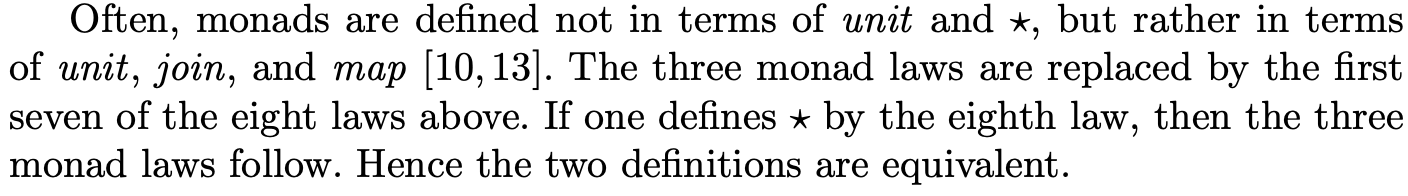
\includegraphics[width=0.6\columnwidth]{wadler-excerpt}\vspace{-0.4\baselineskip}
\par\end{center}

Applicative functors may be defined via \lstinline!ap! and \lstinline!pure!
\emph{or} via \lstinline!map2! and \lstinline!pure!
\begin{itemize}
\item P.~Chuisano and R.~Bjarnason, ``\emph{Functional programming in
Scala}''
\end{itemize}
\begin{center}
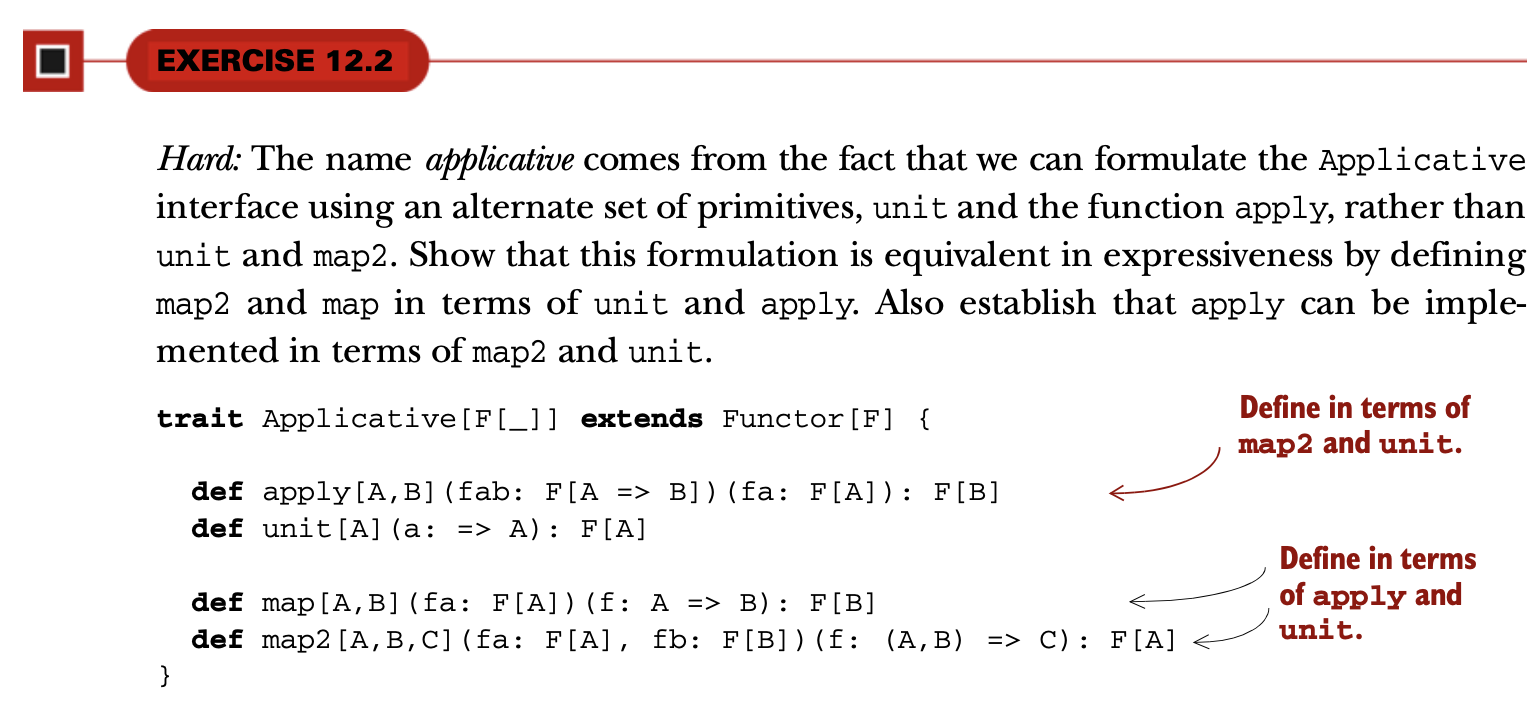
\includegraphics[width=0.45\columnwidth]{fpis-excerpt}\vspace{-0.8\baselineskip}
\par\end{center}

This must be right, but questions remain...
\begin{itemize}
\item What does it mean that \lstinline!x! is ``equivalent in expressiveness''
to \lstinline!y!?
\item How can it be that \lstinline!map2[A, B, C]! is ``equivalent''
to \lstinline!ap[A, B]!?
\end{itemize}
\end{frame}

\begin{frame}{Equivalent formulations of typeclasses II. More examples}

We know that \lstinline!flatMap! is \emph{equal} to the composition
of \lstinline!flatten! and \lstinline!map!

Also, \lstinline!flatten! can be expressed via \lstinline!flatMap!
\begin{lyxcode}
\textcolor{blue}{\footnotesize{}def~flatten{[}A{]}(ffa:~F{[}F{[}A{]}{]}):~F{[}A{]}~=~ffa.flatMap(identity)}{\footnotesize\par}

\textcolor{blue}{\footnotesize{}def~flatMap{[}A,~B{]}(p:~F{[}A{]})(f:~A~=>~F{[}B{]}):~F{[}B{]}~=~p.map(f).flatten}{\footnotesize\par}
\end{lyxcode}
\[
\text{flatten}=\text{flatMap}\left(\text{id}\right)\quad,\quad\quad p\triangleright\text{flatMap}\left(f\right)=p\triangleright f^{\uparrow F}\triangleright\text{flatten}
\]

The \lstinline!pure! method can be expressed via \lstinline!wu!
and vice versa:
\begin{lyxcode}
\textcolor{blue}{\footnotesize{}def~wu:~F{[}Unit{]}~=~pure(())}{\footnotesize\par}

\textcolor{blue}{\footnotesize{}def~pure{[}A{]}(a:~A):~F{[}A{]}~=~wu.map(\_~=>~a)}{\footnotesize\par}
\end{lyxcode}
\[
\text{wu}=\text{pure}(1)\quad,\quad\quad\text{pure}\left(a\right)=\text{wu}\triangleright(\_\rightarrow a)^{\uparrow F}
\]
The \lstinline!filter! method can be expressed via \lstinline!deflate!
and vice versa:
\begin{lyxcode}
\textcolor{blue}{\footnotesize{}def~deflate{[}A{]}(foa:~F{[}Option{[}A{]}{]}):~F{[}A{]}~=}{\footnotesize\par}

\textcolor{blue}{\footnotesize{}~~foa.filter(\_.nonEmpty).map(\_.get)}{\footnotesize\par}

\textcolor{blue}{\footnotesize{}def~filter{[}A{]}(fa:~F{[}A{]})(p:~A~=>~Boolean):~F{[}A{]}~=}{\footnotesize\par}

\textcolor{blue}{\footnotesize{}~~deflate(fa.map~\{~a~=>~if~(p(a))~Some(a)~else~None~\}~)}{\footnotesize\par}
\end{lyxcode}
Notation: $x\triangleright f$ means \lstinline!f(x)! or in Scala
2.13, \lstinline!x.pipe(f)!\\
$f^{\uparrow F}$ means \lstinline!_.map(f)! for the functor \lstinline!F!
\end{frame}

\begin{frame}{Confusing issue 1: ``equivalence'' of values?}

\begin{itemize}
\item Yes, we can express \lstinline!flatten! through \lstinline!flatMap!,
but so what?
\item Is \lstinline!5! ``equivalent'' to \lstinline!10! in expressive
power?
\end{itemize}
\begin{lyxcode}
\textcolor{blue}{\footnotesize{}def~five:~Int~=~ten~/~2}{\footnotesize\par}

\textcolor{blue}{\footnotesize{}def~ten:~Int~=~five~{*}~2}{\footnotesize\par}
\end{lyxcode}
\end{frame}

\begin{frame}{Confusing issue 2: ``equivalence'' of functions with different sets
of type parameters?}
\begin{itemize}
\item How can \lstinline!pure[A]: A => F[A]! and \lstinline!wu: F[Unit]!
be equivalent?
\begin{itemize}
\item An extra type parameter means there are many more implementations
\end{itemize}
\item Example of a \lstinline!pure! that is \emph{not} equivalent to \lstinline!wu!:
\end{itemize}
\begin{lyxcode}
\textcolor{blue}{\footnotesize{}def~badPure{[}A{]}(x:~A):~List{[}A{]}~=~x~match~\{}{\footnotesize\par}

\textcolor{blue}{\footnotesize{}~~case~i:~Int~~~=>~List(i~+~123)}{\footnotesize\par}

\textcolor{blue}{\footnotesize{}~~case~\_~~~~~~~~=>~List(x)}{\footnotesize\par}

\textcolor{blue}{\footnotesize{}\}}{\footnotesize\par}
\end{lyxcode}
\begin{itemize}
\item The corresponding \lstinline!wu = List(())!
\item We cannot restore \lstinline!badPure! from \lstinline!wu!: the corresponding
\lstinline!pure! is \lstinline!List(_)!
\end{itemize}
\end{frame}

\begin{frame}{Equivalence under naturality laws I: example}

The problem with \lstinline!badPure! is that it does not work the
same for all types
\begin{itemize}
\item The code of \lstinline!badPure! is not \textbf{fully parametric}
\item To enforce full parametricity, we require a naturality law: 

\lstinline!pure(f(x)) == pure(x).map(f)!
\[
x\triangleright f\triangleright\text{pure}=x\triangleright\text{pure}\triangleright f^{\uparrow F}\quad,\quad\quad f^{:A\rightarrow B}\bef\text{pure}^{B}=\text{pure}^{A}\bef f^{\uparrow F}
\]

\end{itemize}
\[
\xymatrix{\xyScaleY{2.8pc}\xyScaleX{5.5pc}\mathtt{A}\ar[d]\sb(0.5){~\mathtt{f}}\ar[r]\sp(0.5){\mathtt{pure[A]}} & \mathtt{F[A]}\ar[d]\sp(0.5){\mathtt{\_.map(f)}\text{ for }\mathtt{F}}\\
\mathtt{B}\ar[r]\sp(0.5){\mathtt{pure[B]}} & \mathtt{F[B]}
}
\]

\end{frame}

\begin{frame}{Equivalence under naturality laws II: general formulation}

The precise meaning of the ``equivalent expressive power'' of \lstinline!pure[A]!
and \lstinline!wu!:
\begin{itemize}
\item \vspace{-1\baselineskip}
the set of all functions \lstinline!pure[A]: A => F[A]! satisfying
the naturality law is in a one-to-one correspondence with the set
of all values \lstinline!wu: F[Unit]!
\end{itemize}
Proof:
\begin{enumerate}
\item Start with \lstinline!pure! that satisfies the naturality law; define
\lstinline!wu = pure(())!; then define \lstinline!pure2(x) = wu.map(_ => x)!.
Show that \lstinline!pure2 == pure!:
\begin{align*}
{\color{green}\text{for an arbitrary }x:}\quad & \text{pu}_{2}(x)=\gunderline{\text{wu}}\triangleright(\_\rightarrow x)^{\uparrow F}=1\triangleright\gunderline{\text{pu}\triangleright(\_\rightarrow x)^{\uparrow F}}\\
{\color{green}\text{use naturality law}:}\quad & =\gunderline{1\triangleright(\_\rightarrow x)}\triangleright\text{pu}=x\triangleright\text{pu}=\text{pu}\left(x\right)\quad.
\end{align*}
\item Start with \lstinline!wu: F[Unit]!; define \lstinline!pure(x) = wu.map(_ => x)!;
then define \lstinline!wu2 = pure(())!. Show that \lstinline!wu2 == wu!:
\[
\text{wu}_{2}=\text{pure}\left(1\right)=\text{wu}\triangleright(\gunderline{\_\rightarrow1})^{\uparrow F}=\text{wu}\triangleright\gunderline{\text{id}^{\uparrow F}}=\text{wu}\triangleright\text{id}=\text{wu}
\]
The function \lstinline!pure(x) = wu.map(_ => x)! satisfies the naturality
law:
\begin{align*}
 & \text{pure}\left(x\right)\triangleright f^{\uparrow F}=\text{wu}\triangleright(\_\rightarrow\gunderline{x)^{\uparrow F}\triangleright f^{\uparrow F}}=\text{wu}\triangleright(\_\rightarrow x\triangleright f)^{\uparrow F}\\
 & =\text{wu}\triangleright(\_\rightarrow f(x))^{\uparrow F}=\text{pure}\left(f(x)\right)
\end{align*}
\end{enumerate}
\end{frame}

\begin{frame}{Equivalence under naturality laws III: general pattern}

To prove the equivalence of \lstinline!p: P[A, B, C]! and \lstinline!q: Q[A, B, C]!
under assumption of some naturality laws:
\begin{itemize}
\item Implement functions \lstinline!p2q! and \lstinline!q2p!:
\end{itemize}
\begin{lyxcode}
\textcolor{blue}{\footnotesize{}def~p2q{[}A,~B,~C{]}:~P{[}A,~B,~C{]}~=>~Q{[}A,~B,~C{]}~=~...}{\footnotesize\par}

\textcolor{blue}{\footnotesize{}def~q2p{[}A,~B,~C{]}:~Q{[}A,~B,~C{]}~=>~P{[}A,~B,~C{]}~=~...}{\footnotesize\par}
\end{lyxcode}
\begin{itemize}
\item Show that \lstinline!q2p(p2q(p)) == p! and \lstinline!p2q(q2p(q)) == q!
\item Show that \lstinline!p2q(p)! satisfies \lstinline!q!'s laws, and
\lstinline!q2p(q)! satisfies \lstinline!p!'s laws
\end{itemize}
The ``set of \lstinline!p: P[A, B, C]! satisfying a law'' is a
\textbf{refined type}
\begin{itemize}
\item The Scala compiler cannot verify laws automatically
\item Testing cannot verify laws since type parameters cannot be arbitrary
\item Laws must be verified via symbolic reasoning about code
\end{itemize}
\end{frame}

\begin{frame}{Equivalence under naturality laws IV: further examples}

\begin{itemize}
\item Equivalence of \lstinline!flatten[A]! and \lstinline!flatMap[A, B]!
requires a naturality law for \lstinline!flatMap[A, B]! with respect
to \lstinline!B!
\end{itemize}
\begin{lyxcode}
\textcolor{blue}{\footnotesize{}p.flatMap(f~andThen~g)~==~p.map(f).flatMap(g)}{\footnotesize\par}
\end{lyxcode}
\[
\text{flatMap}\left(f\bef g\right)=f^{\uparrow F}\bef\text{flatMap}\left(g\right)
\]

\begin{itemize}
\item Equivalence of \lstinline!ap! and \lstinline!zip! requires a naturality
law for each of them
\end{itemize}
\begin{lyxcode}
\textcolor{blue}{\footnotesize{}def~ap{[}A,~B{]}:~F{[}A~=>~B{]}~=>~F{[}A{]}~=>~F{[}B{]}~=~...}{\footnotesize\par}

\textcolor{blue}{\footnotesize{}ap(r)(p).map(f)~==~ap(r.map(x~=>~x~andThen~f))(p)}{\footnotesize\par}

\textcolor{blue}{\footnotesize{}def~zip{[}A,~B{]}:~(F{[}A{]},~F{[}B{]})~=>~F{[}(A,~B){]}~=~...}{\footnotesize\par}

\textcolor{blue}{\footnotesize{}zip(p.map(f),~q)~==~zip(p,~q).map~\{~case~(a,~b)~=>~(f(a),~b)~\}}{\footnotesize\par}
\end{lyxcode}
\end{frame}

\begin{frame}{Conclusions}
\begin{itemize}
\item Formulated the ``equivalence of expressive power'' rigorously
\begin{itemize}
\item It is a one-to-one correspondence between\emph{ refined types}
\end{itemize}
\item In most cases, the equivalence holds only after imposing naturality
laws
\item Naturality laws constrain code and may eliminate a type parameter 
\begin{itemize}
\item Naturality laws will hold automatically for fully parametric code
\end{itemize}
\item Functions with simpler type signatures are simpler to reason about
\begin{itemize}
\item Proofs of laws are often easier for \lstinline!flatten! than for
\lstinline!flatMap!
\end{itemize}
\item Full details in the upcoming book --- {\small{}\href{https://github.com/winitzki/sofp}{https://github.com/winitzki/sofp}}{\small\par}
\end{itemize}
\emph{The Science of Functional Programming: A tutorial, with examples
in Scala}

{\small{}}%
\begin{minipage}[t]{0.75\columnwidth}%
\vspace{-0.4\baselineskip}
The book will explain (with examples and exercises):
\begin{itemize}
\item techniques of symbolic reasoning about types
\item techniques for symbolic calculations with code
\item deriving and verifying laws symbolically (as equations for code)
\item real-life motivations for (and applications of) these techniques
\end{itemize}
%
\end{minipage}{\small{}~ }%
\begin{minipage}[t][1\totalheight][c]{0.3\columnwidth}%
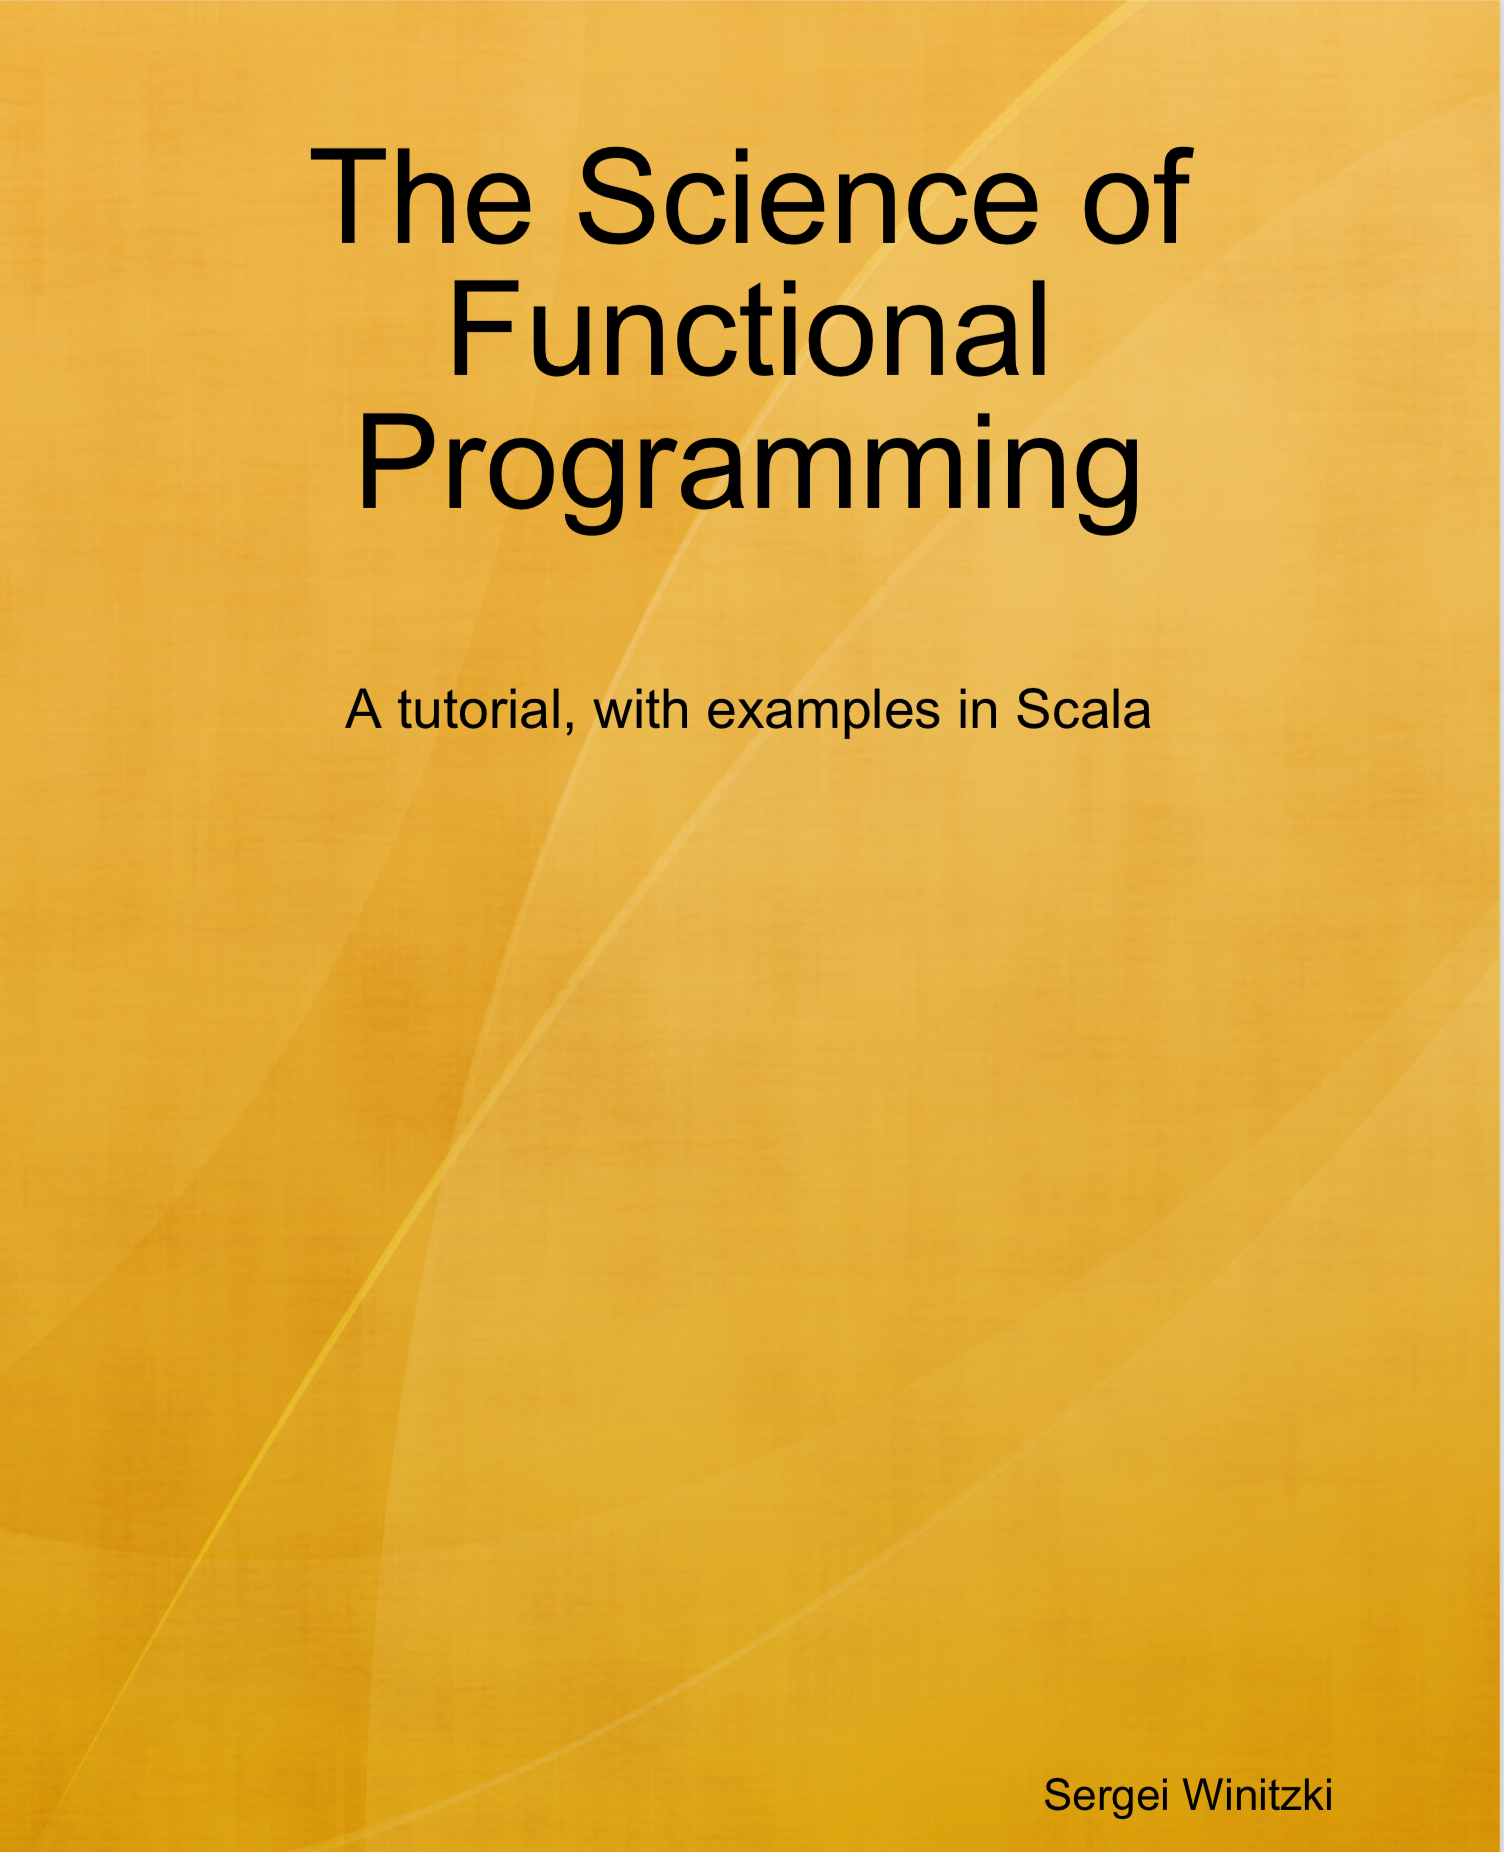
\includegraphics[width=2.5cm]{book-draft-cover}%
\end{minipage}{\small\par}
\end{frame}

\end{document}
